\section{Flow Steering and Processing Allocation Problem}

%%%%%%%%%%%%%%%%%%%
%%%%%%%%%%%
%Basic problem
%%%%%%%%%%%
%%%%%%%%%%%%%%%%%%
\subsection{The basic problem}
\label{subsec:basicproblem}
We begin by introducing the routing and steering problem for the above graph model. In this problem, we are given a \checkthis{directed} graph $G = (V,E)$ along with edge capacities $B : E \rightarrow \positivereal$, vertex capacities $C : V \rightarrow \nonnegativereal$, and a collection of demanded integer flows $D = \{(s_1, t_1, k_1), (s_2, t_2, k_2), \cdots\} \subseteq V \times V \times \positivereal$. While the edge capacities are used in a manner entirely analogous to its uses in standard multicommodity flow problems, we also require that each unit of flow undergo one unit of processing at an intermediate vertex. In particular, while edge capacities limit the \textit{total} amount of flow that may pass through an edge, vertex capacities only bottleneck the amount of processing that may be done at a given vertex, regardless of the total amount of flow that uses the vertex as an intermediate node. \comment[We are then asked to route the flows with minimum congestion, the congestion can be interpreted in 
utilization.]{I don't quite understand this. -YN} \comment{You can ignore this, already covered in your text -KZ} \newtext{The goal is then either to route as much flow as possible, or to satisfy all flow demand subject to appropriate congestion-minimization constraints.} Though ignoring vertex capacity constraints reduces our class of problems to those of the standard Multicommodity Flow variety, the introduction of these constraints forms a new class of problems that (to our knowledge) has not yet been studied in the literature. \comment[Without loss of generality, we assume the flow demand equals processing demand.]{I think this should be moved elsewhere, along with a brief sentence explaining why it's w.l.o.g. -YN} \comment{I think you already covered this part in previous text, KZ} \newtext{Throughout this paper, we make the practice inspired assumption that each unit of flow is in fact an aggregate of many small \textit{\checkthis{microflows}}, and thus all flows are splittable. What can be said about 
this problem subject to unsplittable flow demand remains an interesting open question.} \\

\subsubsection{Flow Maximization}

In \autoref{subsec:maxlps}, we show how to express the maximization version of the problem both as an \textit{edge-based} and as a \textit{path-based} linear program. While neither of these constructions are particularly difficult, it's not immediate that either LP is itself sufficient for solving the problem of identifying the actual routing problem in polynomial time, as the flow-based LP does not identify the individual paths while the path-based LP may end up being of exponential size. In \autoref{subsec:lppaths}, we solve this problem by showing how to construct actual routing patterns from the solution to the edge-based LP. We summarize this result in the following theorem.

\begin{theorem}
\label{thm:flowmax}
There exists a polynomial-sized linear program solving the Maximum Processed Flow problem. Further, the full routing pattern can be extracted from the LP solution in polynomial time. \comment{Should we bother ensuring we don't have bit complexity issues with real numbers? -YN} \comment{KZ: I think the proof takes exponential time, but full routing pattern is contained in the LP solution, in particular, at each node, we take all the incoming flows, divide them into processed and unprocessed, and process part of the unprocessed flow, and then dispense the unprocessed and processed flow based on the flow routing decision $w(e)$ and $f(e)$, but however this approach somehow depends on flow size t and Idk anyway we can get away with it? Seems like if processing of flow is already linear to the flow size, so it may be okay?}
\end{theorem}

Notations:
\newline
For a \emph{path-based} solution, $P_i$: a set of paths $\pi$ for flow $i$; $f(\pi)$: flow size for each path $\pi$ and $p(\pi,v)$: the processing work done at $v$ on path $\pi$.
\newline For an \emph{edge-based} solution, $f_i(e)$: flow size for flow $i$ at edge $e$, $p_i(v)$: the processing work done at v for flow $i$, and $w_i(e)$ is the process work demand at edge $e$ for flow $i$. 

The general linear programming solutions for a multi-commodity flow with in-network processing demand is the following:

\checkthis{Linear programming solution should be totally correct, but you can double check}
\begin{minipage}[t]{0.45\textwidth}
\textit{Path-based formulation:}
  \begin{subequations}
\begin{align}
\text{MAX:}& \sum\limits_{i=1}^K\sum\limits_{\pi\in P_i}f(\pi) \\  \nonumber
\text{Subject } &\text{to:} \\
\forall i,\forall \pi\in P_i; &\sum \limits_{v\in \pi} p(\pi, v) = f(\pi)\\
\forall i,\forall e; \sum\limits_i&\sum \limits_{\pi\in P_i:e\in \pi} f(\pi) \leq B(e)\\
\forall i,\forall v; \sum\limits_i&\sum \limits_{\pi\in P_i: v\in\pi}  p(\pi, v) \leq C(v)\\
\forall i,\forall \pi\in P_i,&\forall v;p(\pi,v) \geq 0
\end{align}
\end{subequations}
  \end{minipage}
\hspace{0cm}
\begin{minipage}[t]{0.50\textwidth}
\textit{Edge-based formulation:}
  \begin{subequations}
\begin{align}
\text{MAX:}&\sum\limits_{i=1}^K\sum \limits_{e=(s,v)} f_i(e)  \\ \nonumber
\text{Subject } &\text{to:}\\
\forall i, \forall v \not= s,t;& \sum\limits_{in}  f_i(e)=  \sum\limits_{out} f_i(e)\\
\forall i,\forall v; p_i(v)& = \sum\limits_{in} w_i(e) - \sum\limits_{out} w_i(e) \\
\forall i,\forall e;  \sum\limits_i& f_i(e)\leq B(e)\\
\forall i,\forall v;  \sum\limits_i& p_i(v) \leq C(v)\\
\forall i,\forall (s\rightarrow v);& w_i (e)= f_i (e)\\
\forall i,\forall (v\rightarrow t);& w_i (e)= 0\\
\forall i,\forall e;w_i (e),& f_i (e)-w_i (e), p_i (v) \geq 0
\end{align}
\end{subequations}
\end{minipage}
\checkthis{Not sure this makes sense to you or not}
The \emph{path-based} solution takes paths as an abstraction, and it captures the properties in an explicit way; the \emph{edge-based} solution, on the other hand can compute the max flow problem in a polynomial time. We further prove that they are equivalent and we can have an path decomposition algorithm to extract the information from \emph{edge-based} solution to formulate the paths. The complexity of this algorithm is similar to Ford-Fulkerson, since we peel off $\Delta f$ at each step.

%%%%%%%%%%%%%%%%%%%
%%%%%%%%%%%
%Flow size change
%%%%%%%%%%%
%%%%%%%%%%%%%%%%%%
\emph{Flow Size Changes after Processing:} the basic max-flow model shows that in-network processing does not affect the traffic volume. However the change of flow size after processing is a common scene in networking, for example, encryption increases the flow size while compression and transcoding decrease the traffic size\cite{Mogul1997}. We can capture this aspect and integrate into the optimization formulation. In a generalized minimum cost circulation problem \cite{Wayne1999}, there is a gaining factor. We apply the same idea, but one key difference in our model is that our model only applies the gaining factor to part of the flow to be processed at a vertex. 

If for flow $i$ there is a size change factor $r_i\in \nonnegativereal$, at each vertex, we have $\sum\limits_{in} w_i(e) - \sum\limits_{out}  w_i(e) = p_i(v)$ and $\sum\limits_{out} (f_i(e) - w_i(e))-\sum\limits_{in}  (f_i(e) - w_i(e))= p_i(v)*r_i$, . If $r_i=1$, we have exactly the flow conservation $\sum\limits_{out} f_i(e) -\sum\limits_{in}  f_i(e)= 0$. 

\subsubsection{Cost Minimization}
\comment{I have a little trouble of telling the difference here, can you elaborate more about the convex function part in this section-KZ}
The minimization version of our problem, however, allows for nonlinear (and, in principle, non-convex) objective functions. In this paper, we deal with the \textit{\checkthis{minimum congestion?}} model, parameterized by two monotone, convex congestion measures $c_v : \nonnegativereal \rightarrow \nonnegativereal$ and $c_e : \nonnegativereal \rightarrow \nonnegativereal$. In this model, a vertex $v$ with processing capacity $C(v)$ is assigned a congestion $c_v(\sum_{f \in F} f_v)$ and each edge is assigned congestion $c_e(\sum_{f \in F} f_e)$, where $f_v$ and $f_e$ are the amount of processing and amount of microflow that flow path $f$ assigns to vertices $v$ and $e$, respectively. Each \textit{\checkthis{microflow}}, in turn, is penalized according to the total amount of congestion it encounters among the edges it takes as well as its processing vertex. \comment[The goal is to feasibly route all requested units of flow while minimizing the sum of the penalties the various \checkthis{microflow} encounter.]{
Since we can turn this problem into a maximization problem with linear objectives with only an $\epsilon$ loss in approximation, shouldn't just about any convex combination of penalties in the objective function be solvable using convex optimization techniques? This captures the minmax problem too, I think... -YN}\comment{Min max is captured by LP already, so yeah this should capture it -KZ}

In terms of optimization formulation, it is very similar to (2.2) \emph{edge-based} solution in section 2.1, however linear constraints (2.2d) and (2.2e) should be removed since they are already captured in the objective function.   



%%%%%%%%%%%%%%%%%%%
%%%%%%%%%%%
%Mutiple tasks as a DAG
%%%%%%%%%%%
%%%%%%%%%%%%%%%%%%
\begin{figure}
 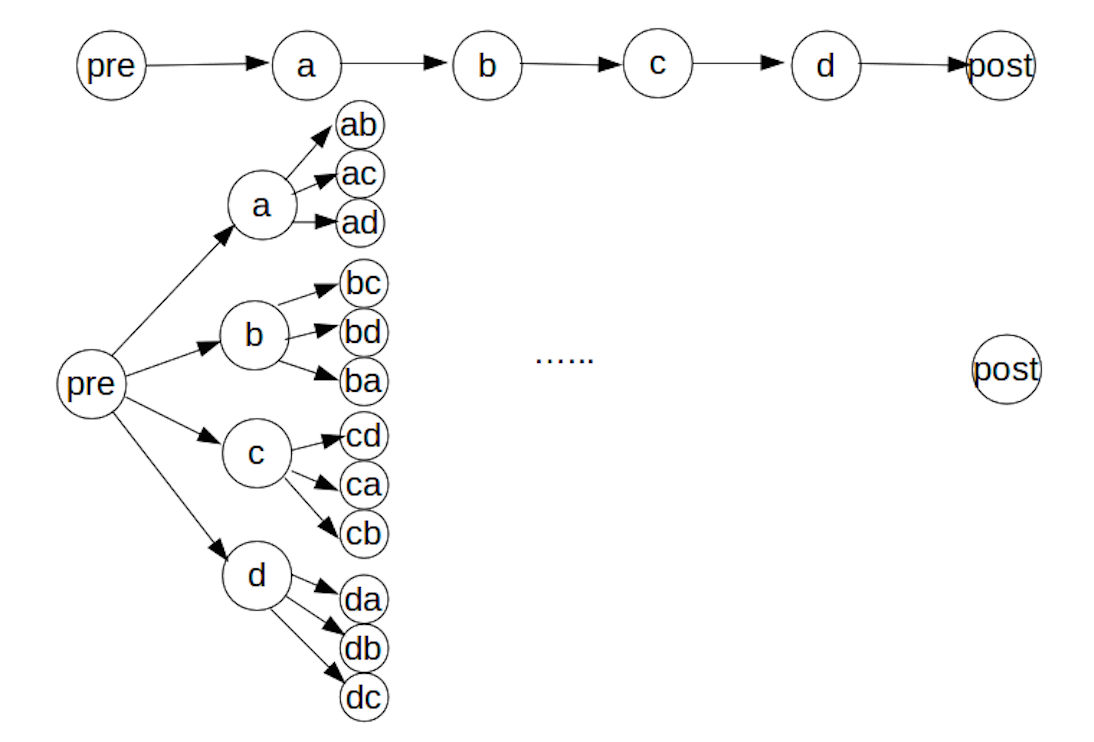
\includegraphics[width=\linewidth]{task.png}
 \caption{up: all serial tasks, Down: all parallel tasks; a,b,c represents three different tasks and each link represents one dependency}
\end{figure}

\subsection{Multiple tasks as a DAG}
In the above formulation we assume either there is only one task, or each vertex can run all types of flow processing tasks where we can bundle all tasks into one task. Nevertheless if we have specialized hardware for different types of tasks or two types of tasks are preferred at different vertices,  we need to revisit our formulation. 
We consider two common types of task relationships: serial and parallel. Serial tasks must be handled in a certain order while parallel tasks can happen in any order. A set of tasks may require a policy of a mixture of serial and parallel, e.g., a flow requires three different types of processing a, b and c, and a is before b and c while b and c can happen in either order. 

We can extract any arbitrary task topology as a partial ordered set (poset). We show two simplest cases where all N tasks are serial or parallel, then we generalize the solution to any arbitrary order via chain-antichain sets.  


For $N$ tasks, we have $C^n(v); n\in\{1\dots N\}$ for $N$ different processing capacities. In optimization formulation 2.2 $f$ and $w$ can be interpreted as two different flow states, pre-processed with volume $w$ and post-processed $f-w$.  In \emph{serial model} we have $N+1$ flow states: pre-$n$-post-$(n-1)$ processed where $ n\in\{1\dots N+1\}$. We can extend formulation 2.2 by adding $N-1$ process demands, in particular for 2.2c we extend to N different types of processing, $p_i^n= \sum\limits_{in} w_i^n(e) - \sum\limits_{out} w_i^n(e)$. Besides the same capacity and flow relation constraints, we also need $w_i^n(e) \geq w_i^{n-1}(e)$ where it reflects the order. The complexity of this formulation increases in a linear relation to the number of tasks $N$. 
In \emph{paralle model} we have $2^N$ processing states and $O(2^N)$ numbers of inequalities for transitioning flow states such as from preprocessed states for cerain tasks to postprocessed states; and $O(N)$ number of inequalities for the vertex capacity.
In general; for a topology with a maximum number of A antichains and L is the maximum length of a chain, then we need maximum $A \lg L$ bits to presents the states, so we have $2^{A \lg L} = L*2^A$ number of states, in other words, the number of flow states is at worst exponential to the width of the poset, and linear to  the height of poset.





%We can satisfy the new requirement by modifying the optimization formulation. We consider two corner cases where there are N serial or N parallel tasks, and then we extend this to a general case where N tasks have a DAG relation. 

%For $N$ serial tasks, we have $C^n(v); n\in\{1\dots N\}$ for $N$ different processing capacities. In optimization formulation 2.2, we can think of two different types of flows, pre-processed and post-processed, and in this model we have $N+1$ types of flows: pre-$n$-post-$(n-1)$ processed where $ n\in\{1\dots N\}$ and  fully processed flows. We can extend formulation 2.2 by adding $N-1$ process demands, in particular for 2.2c we extend to N different types of processing, $p_i^n= \sum\limits_{in} w_i^n(e) - \sum\limits_{out} w_i^n(e)$. Besides the same capacity and flow relation constraints, we also need $w_i^n(e) \geq w_i^{n-1}(e)$ where it reflects the sequence. The complexity of this formulation increases in a linear relation to the number of tasks $N$.


%For $N$ parallel tasks, again we have $C^n(v); n\in\{1\dots N\}$ for $N$ different processing capacities. Unlike serial relation, the number of types of flow grows exponentially, at most there can be $2^N$ types of flows. We have $O(2^N)$ inequalities represents the dependencies and $O(N)$ inequalities represents processing capacity relations.
% Surprisingly the complexity of the formulation also increases in a linear relation to the number of tasks N if we utilize the independence between tasks. The constraints are almost the same as above serial case except for that there is no sequential constraint like $w_i^n(e) \geq w_i^{n-1}(e)$. This optimization problem is similar to solve $N$ separate optimization problems and the $N$ problems are linked by the routing choice $f_i$ and the objective function. We argue that the optimization solution also provides with enough information for routing and processing decision; we can process the flow in the following manner: each flow has $N$ tags which indicates whether the part of the flow $n\in\{1\dots N\}$ is processed, and since the order can be arbitrary for $N$ processings, for each type of processing, it only needs to check its corresponding tag and make decisions independently. 

%To generalize, if there are tasks with a DAG relation where each directed link $(p,q)$ represents a dependency of $q$ to $p$, there is an inequality relation $w_i^q(e) \geq w_i^p(e)$ for each link $(p,q)$. For any k parallel tasks, we need to build $O(2^k)$ branches and establish the relation using the method above.   
